%\documentclass[sigplan,screen]{acmart}
%\documentclass[newfonts=false,format=sigconf,9pt,letterpaper]{acmart}
\documentclass[sigconf,9pt]{acmart}

\usepackage{color}
\usepackage{xspace}
\usepackage{graphicx}
\usepackage{subcaption}
\usepackage[english]{babel}
\usepackage{textcomp}
\usepackage{times}
\usepackage{amsmath}
\usepackage{setspace}
\usepackage[inline]{enumitem}
\usepackage{natbib}
\usepackage{graphicx}
\usepackage[normalem]{ulem}
\usepackage{soul}
\usepackage{latexsym}
\usepackage{bbding}
\usepackage{pbox}

\usepackage{array}
\newcounter{rowcount}
\setcounter{rowcount}{-1}
%MAN: Memory alloc for Networking
%DAMN: Direct Access Memory for Networking
% Segregated Memory N
\newcommand{\oursys}{MAIO\xspace}
\newcommand{\size}{64KB\xspace}
\newcommand{\sockets}{BSD Sockets\xspace}
\newcommand{\X}{\textcolor{red}{\XSolidBrush}}
\newcommand{\V}{\textcolor{green}{\Checkmark}}
\newcommand{\igor}{\textcolor{blue}{IgorY}\xspace}
%%%%%%%%%%%%%%%%%%%%% Commands from prev version
\usepackage[utf8]{inputenc}
\title{Rethinking Zero-Copy Networking with \oursys}

%\author{markuzea Markuze}
%%% potentially enable (i.e. remove the disable command) for the fields below in the camera-ready version          
\settopmatter{printacmref=false}
%\settopmatter{printfolios=false,printacmref=false} %numbers the pages; remove the ugly ACM reference
\setcopyright{none}
\renewcommand\footnotetextcopyrightpermission[1]{} % removes footnote with conference information in first column
\pagestyle{plain} % removes running headers

\begin{document}

\begin{abstract}
    Berkeley Sockets (a.k.a, BSD, POSIX sockets) are ubiquitously used for network communication. \sockets have been the \emph{de-facto} standard API for network I/O since they were introduced almost four decades ago. 
    
    With the advent of high-speed Ethernet, the performance overhead of \sockets became evident. These overheads are particularly burdensome on HTTP proxies and load balancers; their primary operation is to splice TCP sockets, carrying out two operations per network buffer, namely a read and a write. The performance cost of sockets has launched a trend of kernel bypass technologies (e.g., DPDK, AF\_XDP). By bypassing the kernel, these methods attempt to avoid the performance penalties associated with \sockets, i.e., memory copy, system calls, and a slow network stack. However, with great performance comes the great responsibility of re-creating the same network infrastructure that already exists inside the kernel. Kernel developers attempt to close the performance gap by adding new capabilities, most notably AF\_XDP, MSG\_ZEROCOPY, and tcp\_mmap, but none of the proposed solutions is a panacea.
    
    In this work, we propose a new paradigm for userspace networking, aiming to shrink the performance gap between \sockets and kernel bypass techniques, allowing application developers to keep the standard \sockets API, network stack (e.g., TCP) and network tools without compromising on performance. We introduce a \oursys, a dedicated memory allocator for networking which inherently facilitates zero-copy I/O operations and exception-less system calls. \oursys is the first design to provide zero-overhead networking while still taking advantage of the robust kernel network stack without compromising the system's security.
    
    We evaluate a prototype of \oursys, for the use case of TCP socket splicing and compare the performance of \oursys to the state-of-the-art methods. We find that \oursys vastly outperforms standard copying mechanisms like \sockets, and io\_submit and performs on par or better than existing zero-copy techniques while preserving the familiar \sockets API. 
    
\end{abstract}

\maketitle
\sloppypar
%\section{TODO}
%\begin{enumerate}
%    \item Complete Eval.
%    \item Consider Fig with pps and BW on page 1.
%    \item Complete background and table.
%    \item Merge Intro with background?    
%    \item Adjust fig sides.
%\end{enumerate}
\section{Introduction}
\sockets provide a convenient API for user-space I/O, but since their inception network speeds have outstripped those of the CPU. Furthermore, while CPU and memory clock speeds have stagnated in the past decade, Ethernet speeds are growing steadily ~\cite{roadmap}. The greatest performance penalty is due to memory copying, which can take a big part of the CPU cycles ~\cite{desendmsg} and hurt other processes by "polluting" the shared L3 cache and putting additional pressure on the memory channels \cite{markuze2016true}. 

The performance hit due to memory copying is well known. Attempts to ameliorate the costs of moving data have spawn numerous partial optimizations in the kernel (e.g., splice, sednfile, MSG\_ZEROCOPY, tcp\_mmap). A comprehensive solution is missing resulting in the adoption of kernel bypass technologies (e.g., KTCP, Netmap, XDP). Kernel bypass solutions eschew the rich networking infrastructure, developed and perfected in the kernel, leaving the developers with the need to re-develop existing infrastructure (e.g., IP,TCP,ICMP,).

There is a rich literature base spanning 50 years on zero-copy techniques, non provide a full solution (see Related Work). \oursys is an additional step forward towards a usable zero copy technique, that can be applicable both to virtual and physical environments.

\section{Background}
The quest for zero-copy techniques has yielded multiple solutions for zero copy I/O, we will discuss the solutions that are used today (i.e., passed the test of time) and those they may seem related to \oursys. Several previous works have made reviews on zero-copy and fast packet processing techniques\cite{song2012performance,tsiamoura2014survey}. 
\begin{table*}[]
    \centering
    \begin{tabular}{@{\stepcounter{rowcount}\therowcount.)\hspace*{\tabcolsep}}l|c|c|c|c|c|c|l}\hline
        System  & Copy & \pbox{2cm}{System\\Call} & Zero Overhead & \pbox{2cm}{Static\\mapping} & \pbox{2cm}{Network\\ Stack} &  generic use & comments\\\hline
         Naive & 1 & 1 & \X & \V & \V & \V & \\ 
         splice & 0 & 1 & \X & \V & \V & \X & Pipe needed in Linux\\ 
         sendfile & 0 & 1 & \X & \V & \V & \X & Send File only\\ 
         vmsplice & 0 & 1 & \X & \X & \V & \X & No completion notification\\
         SOCKMAP & 0 & 0 & \X & \V & \V & \X & Splicing Only, eBPF\\ 
         io\_map & 0 & 1 & \X & \V & \V & \X & \\ 
         NetMap \cite{rizzo2012netmap} & 0  & 0 & \V & \V & \X & \V &\\
         DPDK \cite{dpdk}& 0 & 0 & \V & \V & \X & \V &\\
         MSG\_ZEROCOPY & 0 & 1 & \X & \X & \V & \V &\\
         tcp\_mmap & 0 & 1 & \X & \X & \V & \X & Full Page size receive\\
         LyraNet & 0 & 1 & \X & \X & \V & \X & \textcolor{red}{\textbf{Please fix wrong lines...}}\\
         INSTANCE & 0 & 1 & \X & \X & \V & \X & Fixed size buffers\\\hline
         RDMA & 0 & 1 & \V & \V & RDMA & RDMA & Specialized HW\\\hline
         \oursys & 0 & 0* & \V & \V & \V & \V &\\\hline
    \end{tabular}
    \caption{Existing Host I/O solutions}
    \label{tab:sol_compare}
\end{table*}

\subsection{eBPF}
XDP,SOCKMAP,io ring.
\subsection{Kernel Bypass}
Netmap,DPDK.
Presumably, when using RAW sockets, \oursys, should behave similarly to NetMap i.e., a shared memory buffer sent/received directly to/from a dedicated TX/RX ring.
NetMap has non standard API, and can never use the Network Stack. Not sure about the message sizes I assume they are fixed or limited in size in NetMap...
We don't have any of these limitations.

\subsection{Socket Splicing - background}
Socket splicing is major area of interest with multiple projects performing HTTP proxy services( \cite{squid,HAProxy,varnish,nginx,ktcp}). To note, NGINX\cite{nginx} and KTCP\cite{ktcp} are used in VMware products.




\section{Design and implementation}
Our main goal when designing \oursys was to preserve a standard \sockets API, while providing seamless zero-copy I/O support. A secondary goal is to eliminate costly system calls from the data path. 

We can classify the existing zero copy techniques into four categories:
\begin{enumerate}
    \item Dynamic remapping (e.g., tcp\_mmap, MSG\_ZEROCOPY\cite{desendmsg}, mikelangelo-project\cite{mikelangelo}).
    \item Kernel Bypass (e.g., DPDK, Netmap\cite{rizzo2012netmap}).
    \item Special/Limited use-case (splice, sendfile).
    \item Shared buffers (e.g, INSTANCE \cite{instance}).
\end{enumerate}
Out of the four categories only \#1 and \#4 allow for a generic use of standard \sockets API. Due to mainly security concerns examples that fit into category \#4 are the rarest.
While there are many examples to solutions that fall into category \#1 \cite{mikelangelo-empty,desendmsg}, but they usually discover that modifying virtual memory on the fly is computationally expensive. 

For these reasons we have decided that we should look into a Shared buffer solution. Our inspiration for a correct shared buffer solution comes from a similar problem in IOMMU security. DAMN \cite{markuze2018damn}, creates a memory allocator based on a pool of perpetually DMA mapped buffers, which are used for I/O by the Linux Network stack and device drivers. This solution effectively creates a \emph{secure} shared memory solution between the Server and the NIC.

We propose \oursys, a Memory Allocator for I/O, for the  exclusive use of the network stack. The \oursys allocator uses a pool of dedicated compound memory pages(i.e., \_\_GFP\_COMP). We adopt the allocation mechanics proposed in DAMN\cite{markuze2018damn}. I.e., the allocator is based on two known mechanisms; a page\_frag mechanism \cite{pagefrag} over \size buffers, these buffers in turn are allotted by a magazine allocator \cite{bonwick2001magazines}. This allocation scheme allows for efficient allocation of variable size buffers in the kernel. Variable size allocations is needed to support variable sizes of MTU and HW offloads (e.g., HW GRO). 
To facilitate zero copy, these pages are mapped \emph{once} to the virtual memory address space of the privileged user-space process. In order to use \oursys, the user-space program, has to mmap the \oursys buffer and then allocate a virtual region for its own use (i.e., zero-copy send), the size of the allocated region should be a multiple of \size. A second way the user-space process can get \oursys buffers, is by performing zero-copy receive. The user-space process can return memory to the kernel via a exception-less mechanism described in Sec. \ref{sec:bifurcated}.
The \oursys buffers are depicted in Fig. \ref{fig:our_sys} as dashed boxes.
%That process is now able of perform zero-copy I/O.
\subsection{Bifurcated I/O}\label{sec:bifurcated}
A second issue that impacts user space I/O performance, is the direct and indirect cost of system calls\cite{flexsc}.
To avoid the costly operation of invoking a costly system calls we offload the I/O operation to a dedicated kernel thread (Fig. \ref{fig:our_sys} \textbf{(3)}) which will perform the I/O operation using kernel sockets \cite{ktcp}. For example a \texttt{send\_msg} system call is replaced with an I/O descriptor (i.e., \texttt{struct msghdr} and \texttt{int flags}) written to a shared memory ring buffer (Fig. \ref{fig:our_sys} \textbf{(2)}).
%RX: just poll the descriptor ring or sleep with sys call.
%TX: continuous poll. NAPI like execution, with amortized sys call, when not polling.


\subsection{Security}
Such a solution initially razes concerns about the security and stability of the system, as the process now \emph{seemingly} has access to sensitive kernel memory. 

\noindent\textbf{Driver Support.} We can allocate dedicated NIC RX rings for \oursys users. HW support\cite{flow_direct} can direct a single 5 tuple (or a defined group of 5 tuples). Limiting the shared buffers \emph{only} to this users data. The implementation of a driver support, is out of the scope of this work. 

\noindent\textbf{Kernel Security.} \oursys is integrated in such a way that the shared pages are only ever used by the Kernel to hold the I/O \emph{data} buffers and \emph{not} the meta data or any other kernel need. Namely, the process can only ever see the information it has written or data bound to user-space. In addition to the data, the process is privy to the transport headers as well; we assume the NIC supports Header/Data splitting\cite{hds} which can place the headers onto non-shared buffers.

\noindent\textbf{User Security.} By sharing all potential RX buffers \oursys exposes all traffic to a single observer.
Without driver support this limits the usefulness of \oursys to those cases when the user is trusted (e.g., sudo). 

\subsection{Shared buffer concerns.}
\noindent\textbf{Kernel Starvation.} The user process may hoard \oursys buffers without releasing them to the kernel.
In this case the dri


\noindent\textbf{Pinned pages.} In early solutions proposed for zero-copy by shared static buffer, were considered dangerous because these shared pages can be exhausted and cannot be swapped out \cite{song2012performance,yamagiwa2005active}. We contend that this is not a real concern for modern systems as systems with hundreds of GB are the norm. Key/Value applications (e.g., memcached, redis) expect their memory to be persistent in memory. Additionally HPC applications, many\cite{top500} of which use RDMA, \texttt{register} (i.e., pin to memory) large memory regions that are then used for I/O.

\subsection{zero copy support for kernel sockets}
We expand the existing Linux TCP API with a \texttt{tcp\_read\_sock\_zcopy} for \texttt{RX} and add a new msg flag \texttt{SOCK\_KERN\_ZEROCOPY} for \texttt{tcp\_sendmsg\_locked} in \texttt{TX}. We base our new function \texttt{tcp\_read\_sock\_zcopy} on existing infrastructure i.e., \texttt{tcp\_read\_sock}. It is used by \texttt{tcp\_splice\_read} to collect buffers from a socket without copying. For \texttt{TX}, zero copy infrastructure already exists in the form of MSG\_ZEROCOPY\cite{desendmsg}. When kernel memory is used for I/O, enabling zero copy is trivial when compared to zero copy from user space. The pages are already pinned in memory and there is not need for a notification on \texttt{TX} completion. The pages are reference counted, and can be freed by the device driver completion handler.

\subsection{Virtual Environment: Future/Related...}
TODO: Virto does dynamic re-mapping, some papers also exist on kvm by the same people of "mikelangelo" \cite{mikelangelo}. Need to look at VMXNET3 code...

\begin{figure}[t]
    \centering
    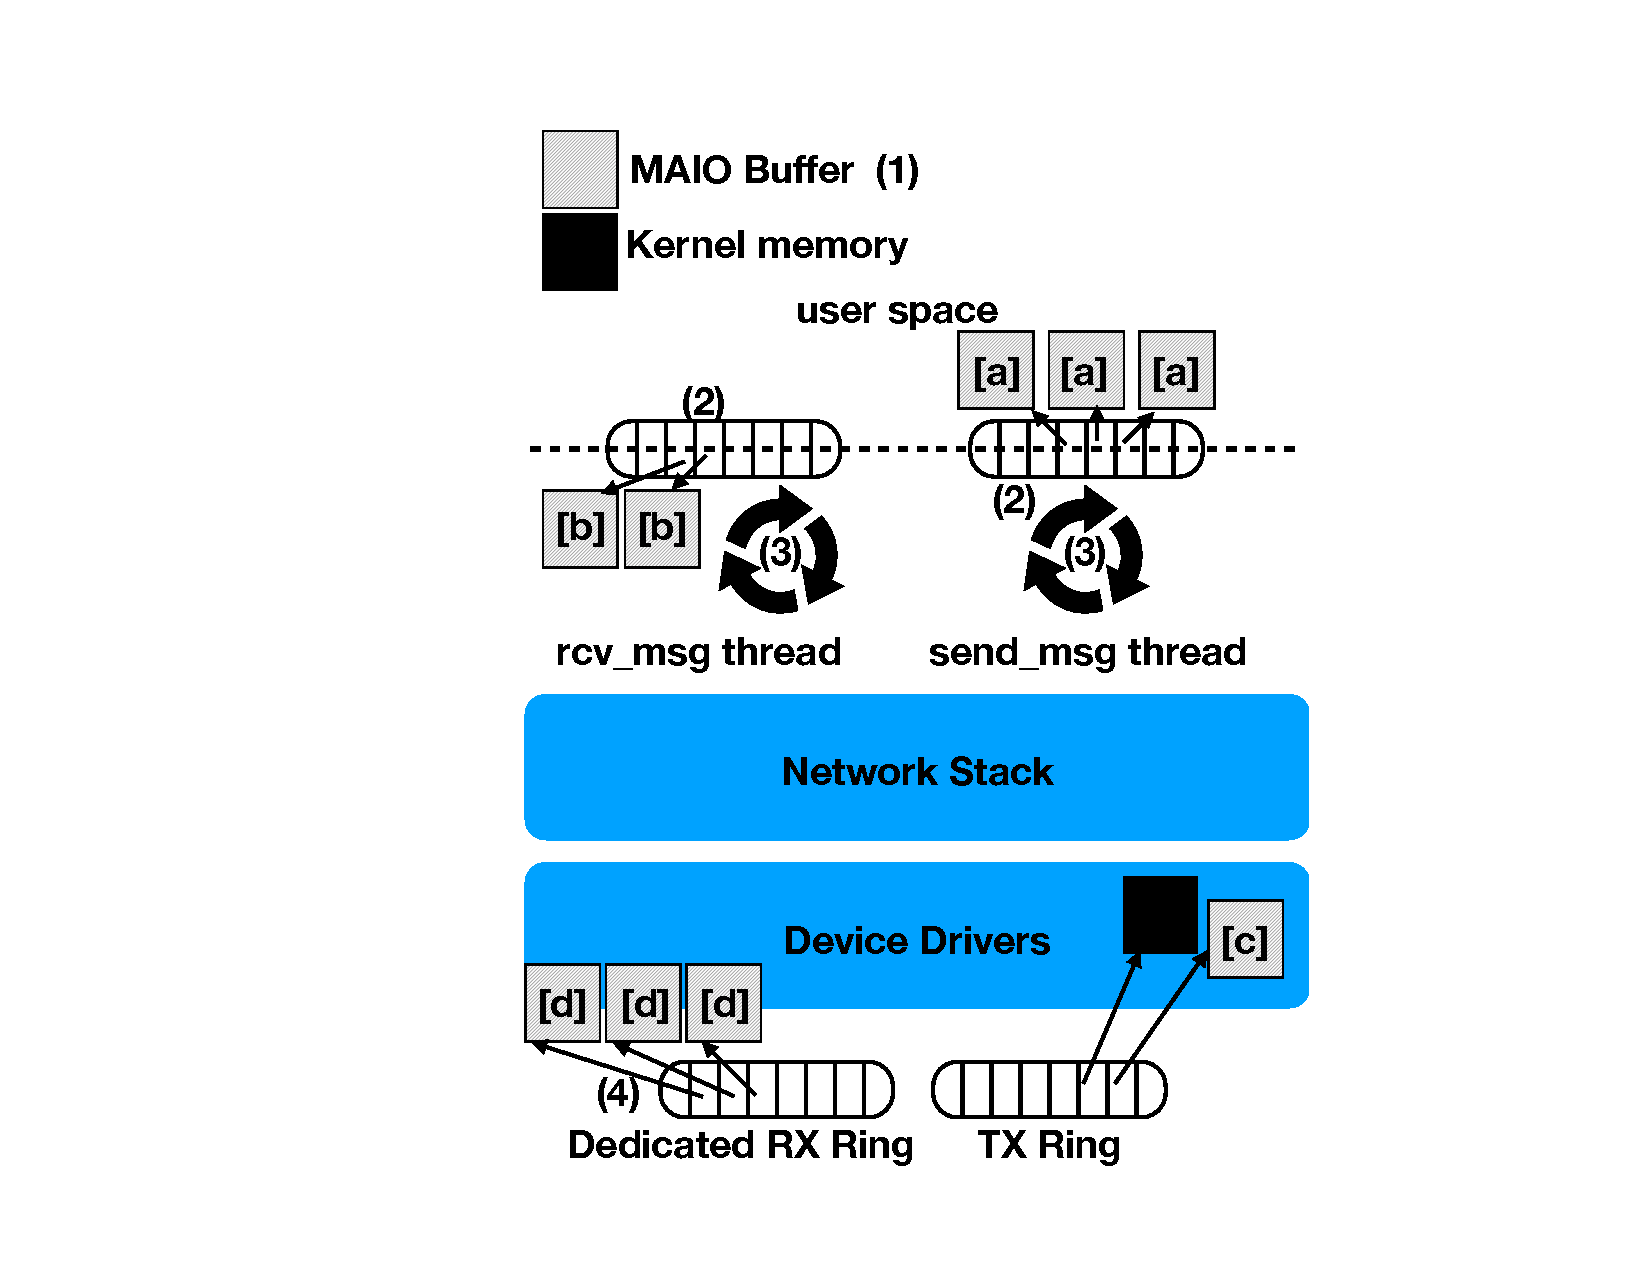
\includegraphics[width=0.8\columnwidth]{ktcp_z.pdf}
    \caption{1. \oursys shared memory buffers 2. shared io rings for exception-less system calls 3. A kernel thread executing I/O operations 4. A dedicated RX ring.
    [a] zero-copy send\_msg [b] zero-copy recvmsg [c] \oursys buffer in driver TX ring [d] \oursys buffers used by the device driver for RX}
    \label{fig:our_sys}
\end{figure}
%Related to FlexSC \cite{flexsc}, \\TODO:\\
%1. ~/memory\_trace/poller/\\
%2. rerun context switch tests?
\begin{figure}[t]
    \centering
    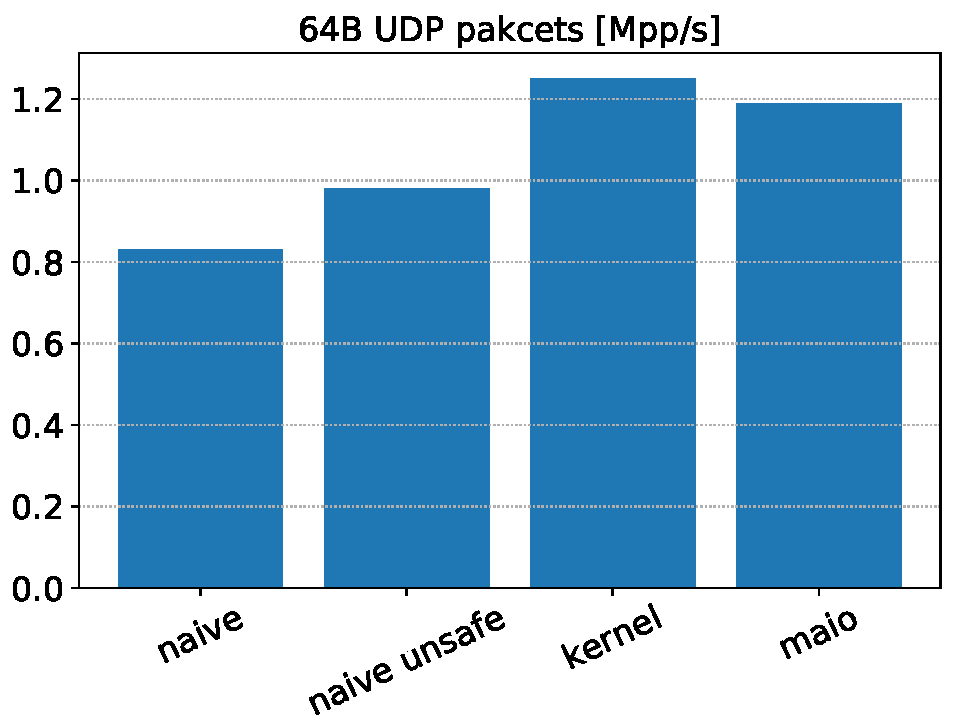
\includegraphics[width=\columnwidth]{syscall.pdf}
    \caption{Number of 64B udp packets sent using user-space sockets(both with and without mitigations), kernel sockets and MAIO.} 
    \label{fig:pps}
\end{figure}
\begin{figure}[t]
    \centering
    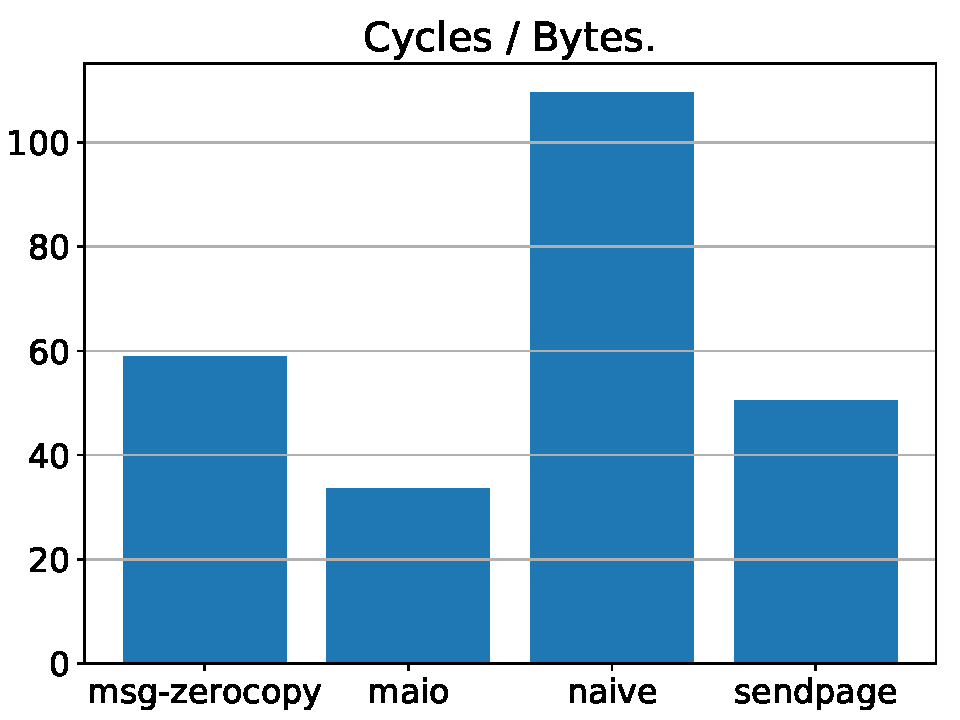
\includegraphics[width=\columnwidth]{send.pdf}
    \caption{The average cycles per packet needed for each zero-copy method (16KB sends). [lower is better]}
    \label{fig:tx_compare}
\end{figure}
\section{Evaluation}\label{sec:eval}
We evaluate the benefits of \oursys on a virtual environment in the Google Clod Platform(GCP).
For our testing we have crated three VMs; 16 core\footnote{These VMs have two threads per physical core} Intel Cascade Lake high-throughput VMs capable of 32Gb/s of egress bandwidth\cite{gcp}, each with 64GB of RAM.

In all experiments we have repeated the test 10 times, and we show the average result. We use perf\cite{perf} to analyze the major contributors to the cycles per byte costs of each of tested techniques.

\subsection{Bifurcated TX}\label{sec:eval_bif}
In this experiment we evaluate the direct benefit of bifurcated system calls. Each program sends a UDP stream of 64 Byte packets. The goal of this experiment is to gauge the impact of system calls on performance. We compare a simple \texttt{send\_msg}, a kernel thread performing \texttt{kernel\_send\_msg} and \oursys. We run the naive version twice, once with \texttt{mitigations=off}\cite{mitigations} and once without this boot parameter. We present the number of sent datagrams per second in million packets per second(Mpp/s), the results are shown in Fig \ref{fig:pps}. We see that \texttt{mitigations}(naive unsafe in the figure) have a negative impact of 20\% on the performance of the naive \texttt{send\_msg}. Without mitigations a kernel thread and \oursys still perform better than the naive thread by 25\% and 20\% respectively.

\subsection{Zero Copy TX}
We evaluate the cost of data copying for single sending process. To minimise the impact of system calls on performance we send 16KB buffers. We evaluate a simple \texttt{send\_msg}(i.e., naive), a \texttt{send\_msg} with the \texttt{MSG\_ZERO\_COPY} flag, \texttt{sendfile} and \oursys. In this experiment all the senders were working at the rate of 27Gb/s, but the \texttt{send\_msg}, which was bottle necked on the core CPU and as a result working at the rate of 19Gb/s. The results of the experiment are shown in Fig. \ref{fig:tx_compare}, we show the Cycles/Byte metric as a meter of efficiency. We calculate the metric by measuring the CPU utilisation in CPU cycles and dividing by the total bytes sent per second. In this experiment about 50\% of the CPU cycles for \texttt{send\_msg} were spent on copying data. This amounts to about 55 CPU cycles spent on each sent Byte, we assume this includes memory access. With the \texttt{MSG\_ZERO\_COPY} flag, about 37\% of the CPU cycles are spent on \texttt{get\_user\_pages\_fast}, which translates to 22 cycles spent on dynamic remapping per byte. These results confirm the findings first reported in the original \texttt{MSG\_ZERO\_COPY} paper\cite{desendmsg}. Sendpage, was closer in performance numbers to \texttt{MSG\_ZERO\_COPY} rather than to \oursys, due to the cost of \texttt{splice} abstractions, with 19\% of the cycles spent on \texttt{generic\_file\_splice\_read} and another 7\% spent on call stack from \texttt{generic\_splice\_sendpage} to the actual \texttt{tcp\_sendpage} that performs the TCP send. In the Linux kernel \texttt{send\_msg} is implemented with \texttt{splice} abstractions.

\begin{figure}[t]
    \centering
    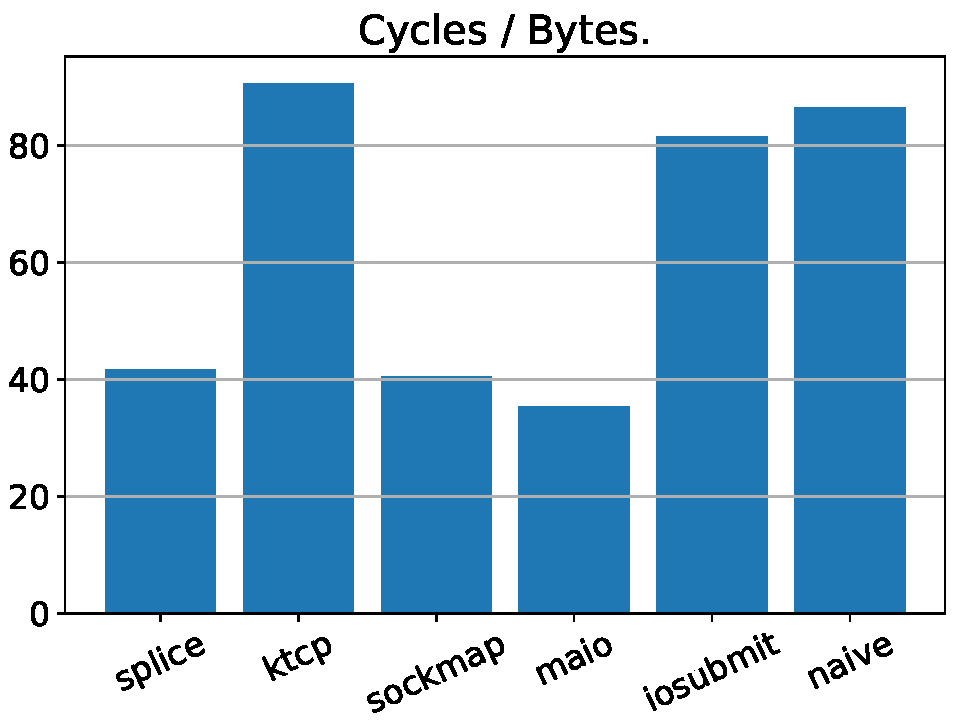
\includegraphics[width=\columnwidth]{splice.pdf}
    \caption{The average cycles per packet needed for each splicing solution. [lower is better]}
    \label{fig:cyc_byte}
\end{figure}

\subsection{Socket Splicing}
We perform a simple TCP socket splicing experiment (i.e., Moving bytes from one TCP socket to another) akin to the TCP-split functionality of KTCP. We measure the effectiveness of each proposed solution by looking the the number of CPU cycles spent on average to splice (i.e., receive and send) a single byte. In this experiment we compare \oursys to user-space proxies implemented with splice\cite{splice}, iosubmit\cite{cloudflare_aio} and \sockets and also to KTCP\cite{ktcp} and SOCKMAP\cite{sockmap}. Results of the experiment are shown in Fig. \ref{fig:cyc_byte}.

We use 256KB buffers both for RX and TX, rendering the effect of system calls negligible. System calls account for less than 1\% of the cpu syscalls of iosubmit,splice and naive. Unsurprisingly, KTCP, iosubmit and naive all spend between 25\% to 32\% of the cycles on memory copying. While both splice and sockmap perform much better than the copying functions \oursys is still able outperform both by about 10\%. \oursys has none of the \texttt{splice} abstraction overheads between the actual TCP receive and send and none of the costs associated with eBPF. 

%Why we are \emph{not} touching DPDK and friends with a stick.

%Splice Compare (Check Poll):
%\begin{itemize}
%    \item Naive
%    \item SOCKMAP
%    \item splice
%    \item vmsplice  (?)
%    \item io\_remap (?)
%    \item ktcp - kernel TCP client + halfduplex.
%    \item \oursys - kernel zero TCP client + read/write op. 
%    \item ktcp\_zero. - kernel zero TCP client
%\end{itemize}


%\subsection{BW - cycles/byte}
%\subsection{Latency TCP/RR}
%\subsection{Scale - multiple connections - BW,Latency}

\section{Related Work}
Review of zcopy techniques:\\
\url{http://www.cscjournals.org/manuscript/Journals/IJCSS/Volume6/Issue4/IJCSS-756.pdf}\\
Lyranet:\\
\url{https://webpages.uncc.edu/~jmconrad/EmbeddedSystems/TCP_IP\%20protocol\%20stack.pdf}\\
Instance:\\
\url{https://heim.ifi.uio.no/paalh/instance/espen.pdf}\\
ZeroCopy Paravirt:\\
\url{https://events19.linuxfoundation.org/wp-content/uploads/2017/12/Empty-Promise-Zero-Copy-Receive-for-vhost-Mike-Rapoport-IBM.pdf}

\section{Future Work}
We plan on testing a full version of \oursys kernel including a dedicated RX buffer support on a physical setup. With that implementation, we plan on testing the performance benefit for real user applications beyond socket splicing (e.g., Memcached).

Also, we are keen on exploring the potential benefits of \oursys a para-virtual system. We believe, that a perpetual exposure of dedicated host memory can be a boon to para-virtual networking. Potentially allowing for full zero-copy I/O from the user-space of a guest OS.
\section{Conclusion}
In this work, we have presented \oursys, a novel paradigm for user-space networking. \oursys facilitates zero-overhead network I/O, i.e., zero-copy and exception-less system calls. Unlike previous solutions, \oursys preservers the ubiquitous \sockets API without sacrificing the system's performance or safety.
%There is a rich literature base spanning 50 years on zero-copy techniques, non provide a full solution\cite{song2012performance}. 
\oursys is a much-needed step forward towards a performant and generic zero-copy technique. %A solution that we presume can be applied both to virtual and physical environments.
%We Rule.
%``I always thought something was fundamentally wrong with the universe'' \citep{adams1995hitchhiker}

\bibliographystyle{plain}
\bibliography{references}
\end{document}
